\subsection{BPD}
BPD which means backward proton detector was developed for the measurement of backward proton decay from $\Lambda$ in $Y^*\rightarrow \pi^0 \Sigma^0 \rightarrow \pi^0 \gamma \pi^0 \Lambda$ decay scheme
which was installed at most upstream of the CDS.
The scattered angle of $Y^*$ is enhanced backward scattering, especially below the threshold due to small momentum transfer.
The BPD was installed to obtain large acceptance for these protons.
The BPD is a plastic scintillator hodoscope array with a size of 350mm (horizontal) $\times$  340mm (vertical).
It is segmented into 70 units of 5mm $\times$ 5mm $\times$ 340mm scintillation counter made of Eljen EJ-230.
Two MPPCs with a 3mm$\times$3mmm sensitive area (Hamamatsu S10362-33-050C) were directly put on both sides of each slab.
The present thesis explains the $\pi^{\mp}\Sigma^{\pm}$ and the $d(K^-, p)"\pi^-\Sigma^0"$ modes analysis,
so BPD was used only energy loss calculation.

\subsection{Vertex chamber - BPC}
\begin{figure}[htbp]
  \centering
  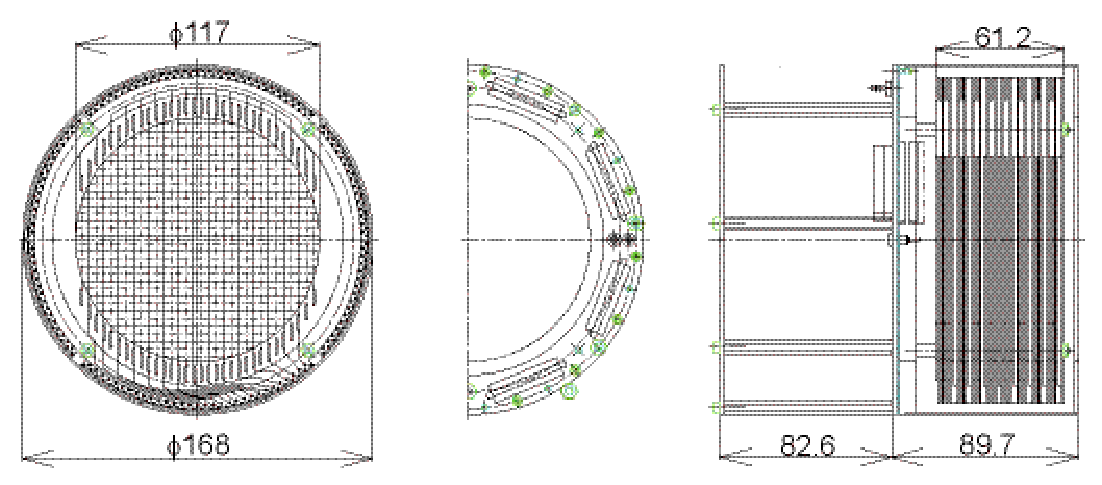
\includegraphics[width=9cm]{pic/experiment/BPC_Run68.eps}
  \includegraphics[width=9cm]{pic/experiment/BPC.png}
  \caption{
    Schematic view of the BPC. Above figure shows about MR-RUN69.
    Bottom figure shows about MR-RUN78.
  }
  \label{fig:BPC}
\end{figure}
BPC which means backward proton chamber was developed for the measurement of backward proton decayed from hyperons that come from $\pi^0\Sigma^0$ mode.
The BPC also used beam tracking at just upstream of the experimental target for the definition of reaction vertex point.
The BPC was installed at just upstream of the experimental target where is in the CDS described after.
The BPC is a planer type drift chamber which has a circular plane to maximize effective area in limited space.
The BPC configuration is XX'YY'XX'YY', so the BPC has 8 layers.

In MR RUN69, the chamber with 168mm diameter outer which has 15 sense wires per layer with 3.6mm drift length corresponding to 111.6mm effective area was used as the BPC.
In this run, the inner hodoscope (IH) was installed in CDS for the trigger counter to evaluate CDC efficiency.

In MR RUN78,the IH was removed to maximize acceptance of backward proton so larger chamber was used as the BPC
whose outer size is 290mm diameter and 32 sense wires per layer with 3.0mm drift length corresponding to 189mm effective area.

These chambers were used 50$\mu$m diameter copper-beryllium wire for potential wires and 12.5$\mu$m diameter gold-plated tungsten.
These cathode planes are made of 9$\mu$m carbon aramid foil.
These are 120 read-outs and 256 read-outs in MR-RUN69 and MR-RUN78, respectively.

